\documentclass[11pt,a4paper]{article}
\usepackage[utf8]{inputenc}
\usepackage[T1]{fontenc}
\usepackage{lmodern}
\usepackage{amsmath, amsfonts, amssymb}
\usepackage{graphicx}
\usepackage{geometry}
\geometry{margin=1in}
\usepackage[hidelinks]{hyperref}
\usepackage{booktabs}
\usepackage{array}
\usepackage{parskip}
\usepackage{tikz}
\usepackage{caption}
\usepackage{float}
\usepackage{subcaption}
\usepackage{xcolor}

\graphicspath{{../results/figures/}}

\definecolor{gdblue}{HTML}{1565C0}
\definecolor{gaorange}{HTML}{E65100}

\title{Technical Report:\\GD vs GA for Urban Sound Classification}
\author{Custom Smart Adaptive Systems $\cdot$ UPC 2025/26}
\date{\today}

\begin{document}
\maketitle

\begin{abstract}
This report compares two fundamentally different methods for training a Multilayer Perceptron (MLP)
for urban sound classification: Gradient Descent (GD) using the Adam optimizer and a Genetic
Algorithm (GA) using the DEAP library. Both methods optimise the same 2,710-parameter MLP on the
UrbanSound8K tabular dataset. Hyperparameters are tuned independently with Optuna (TPE). GD achieves
a test accuracy of 88.7\% in approximately 52 seconds. The GA reaches 61.2\% in approximately 155
seconds. The report details the methodology, core design decisions, and a direct performance
comparison between gradient-based and evolutionary weight optimisation.
\end{abstract}

\tableofcontents
\newpage

% ─────────────────────────────────────────────────────────────────────────────
\section{Introduction}
% ─────────────────────────────────────────────────────────────────────────────

Neural networks are conventionally trained by gradient descent, which follows the gradient downhill
in loss space and scales well to millions of parameters. This project explores an alternative:
evolving the network's weight vectors using a Genetic Algorithm (GA), a population-based
metaheuristic that requires no gradient information whatsoever.

The experimental design deliberately holds the architecture constant: the exact same MLP with the
exact same 2,710 parameters is handed to both optimisers. Only the training mechanism differs. This
isolates the effect of the optimisation strategy and enables a clean comparison of accuracy,
convergence behaviour, and wall-clock time on a 10-class urban sound classification task.

% ─────────────────────────────────────────────────────────────────────────────
\section{Methodology}
% ─────────────────────────────────────────────────────────────────────────────

\subsection{Dataset}

The UrbanSound8K tabular dataset contains 8,674 pre-extracted audio feature vectors distributed
across 10 urban sound classes (air conditioner, car horn, children playing, dog bark, drilling,
engine idling, gun shot, jackhammer, siren, street music). Each sample consists of 34 numerical
features standard in audio machine learning:

\begin{itemize}
    \item \textbf{MFCC (13):} Mel-frequency cepstral coefficients capturing the spectral envelope.
    \item \textbf{Chroma (12):} Pitch-class energy distribution.
    \item \textbf{Spectral Contrast (7):} Ratio of spectral peaks to valleys.
    \item \textbf{Zero Crossing Rate (1):} Proxy for signal noisiness.
    \item \textbf{Spectral Centroid (1):} Brightness indicator.
\end{itemize}

\begin{figure}[H]
    \centering
    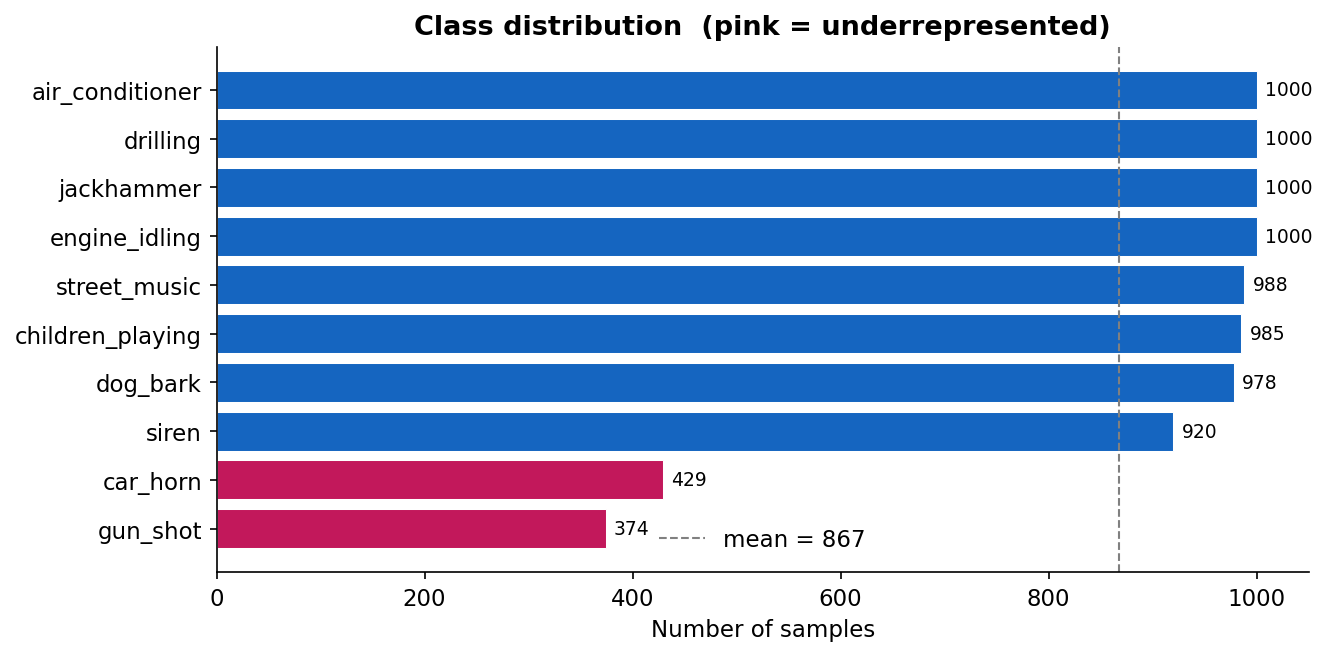
\includegraphics[width=0.80\textwidth]{class_distribution.png}
    \caption{Class distribution across the 10 urban sound categories. Car horn and gun shot are
    underrepresented ($<$300 samples), motivating stratified splitting.}
    \label{fig:class_dist}
\end{figure}

\subsection{Preprocessing}

Each of the 34 features is standardised to zero mean and unit variance using
\texttt{StandardScaler} fit only on the training split. This prevents larger-magnitude features
(e.g.\ spectral centroid) from artificially dominating weight updates during GD, and ensures the GA
fitness landscape is similarly scaled.

The dataset is split stratified by class: 70\% train (6,072 samples), 10\% validation
(867 samples), 20\% test (1,734 samples). Stratification ensures that the two
underrepresented classes (car horn, gun shot) appear in all three splits proportionally.

\begin{figure}[H]
    \centering
    \begin{subfigure}[b]{0.48\textwidth}
        \centering
        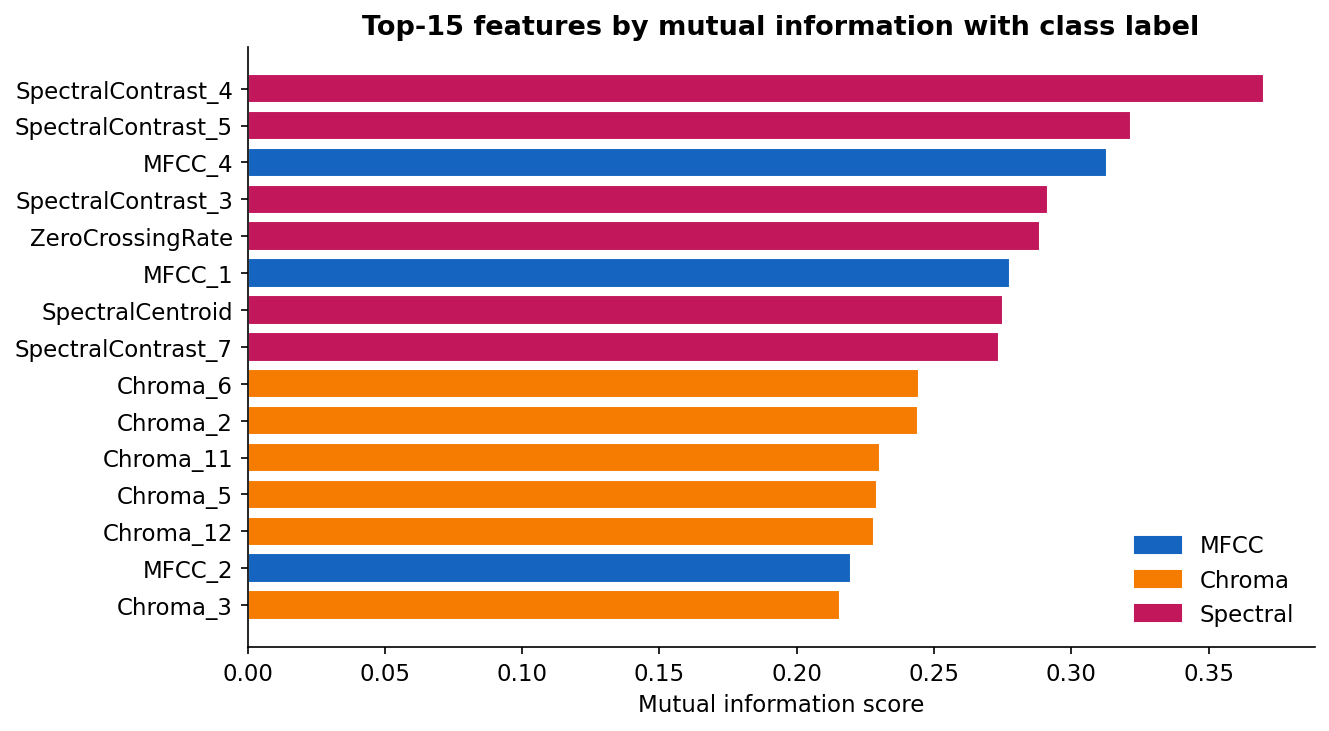
\includegraphics[width=\textwidth]{feature_importance.png}
        \caption{Mutual information scores for each of the 34 features.}
        \label{fig:feat_imp}
    \end{subfigure}
    \hfill
    \begin{subfigure}[b]{0.48\textwidth}
        \centering
        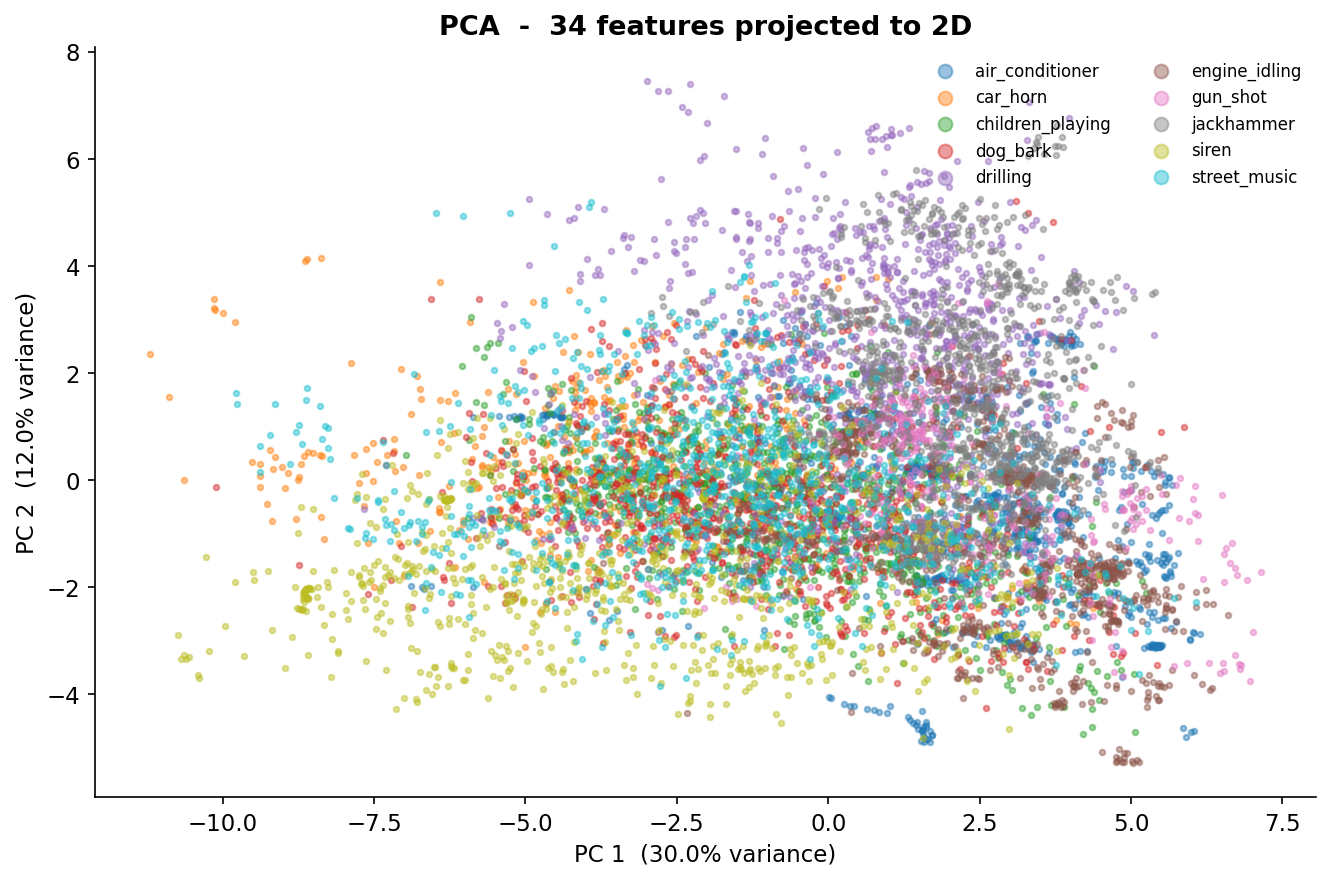
\includegraphics[width=\textwidth]{pca_2d.png}
        \caption{2D PCA projection (PC1+PC2 explain $\approx$42\% of variance).}
        \label{fig:pca}
    \end{subfigure}
    \caption{Feature analysis. Heavy class overlap in the PCA projection justifies a non-linear
    ReLU-activated MLP over a linear classifier.}
    \label{fig:feature_analysis}
\end{figure}

% ─────────────────────────────────────────────────────────────────────────────
\section{Network Architecture}
% ─────────────────────────────────────────────────────────────────────────────

The network is a fully-connected MLP implemented in PyTorch:

\[
  \mathbf{h} = \mathrm{ReLU}(\mathbf{W}_1\mathbf{x} + \mathbf{b}_1), \qquad
  \hat{\mathbf{y}} = \mathbf{W}_2\mathbf{h} + \mathbf{b}_2
\]

\noindent with input dimension 34, hidden dimension 60 (Optuna-tuned), and output dimension 10.
The total parameter count is:

\[
  (34 \times 60 + 60) + (60 \times 10 + 10) = 2{,}100 + 610 = 2{,}710 \text{ parameters}
\]

PyTorch was chosen over scikit-learn's \texttt{MLPClassifier} because it provides direct
read/write access to the flat weight vector via \texttt{torch.nn.utils}. The GA exploits
this to extract and inject all 2,710 weights as a single flat array in microseconds,
with no gradient tape or optimiser state overhead during fitness evaluation.

% ─────────────────────────────────────────────────────────────────────────────
\section{Training Approaches}
% ─────────────────────────────────────────────────────────────────────────────

\subsection{Gradient Descent (GD)}

The GD model is trained with the Adam optimiser minimising cross-entropy loss:

\[
  \mathcal{L} = -\frac{1}{N}\sum_{i=1}^{N}\sum_{c=1}^{10} y_{ic}\log\hat{y}_{ic}
\]

Tuned hyperparameters (Optuna, 60 trials): learning rate $\eta = 4.96 \times 10^{-3}$, weight
decay $\lambda = 3.29 \times 10^{-5}$, hidden dimension $h = 60$. Training runs for a maximum of
150 epochs with early stopping (patience 10). Batch size is 64.

\begin{figure}[H]
    \centering
    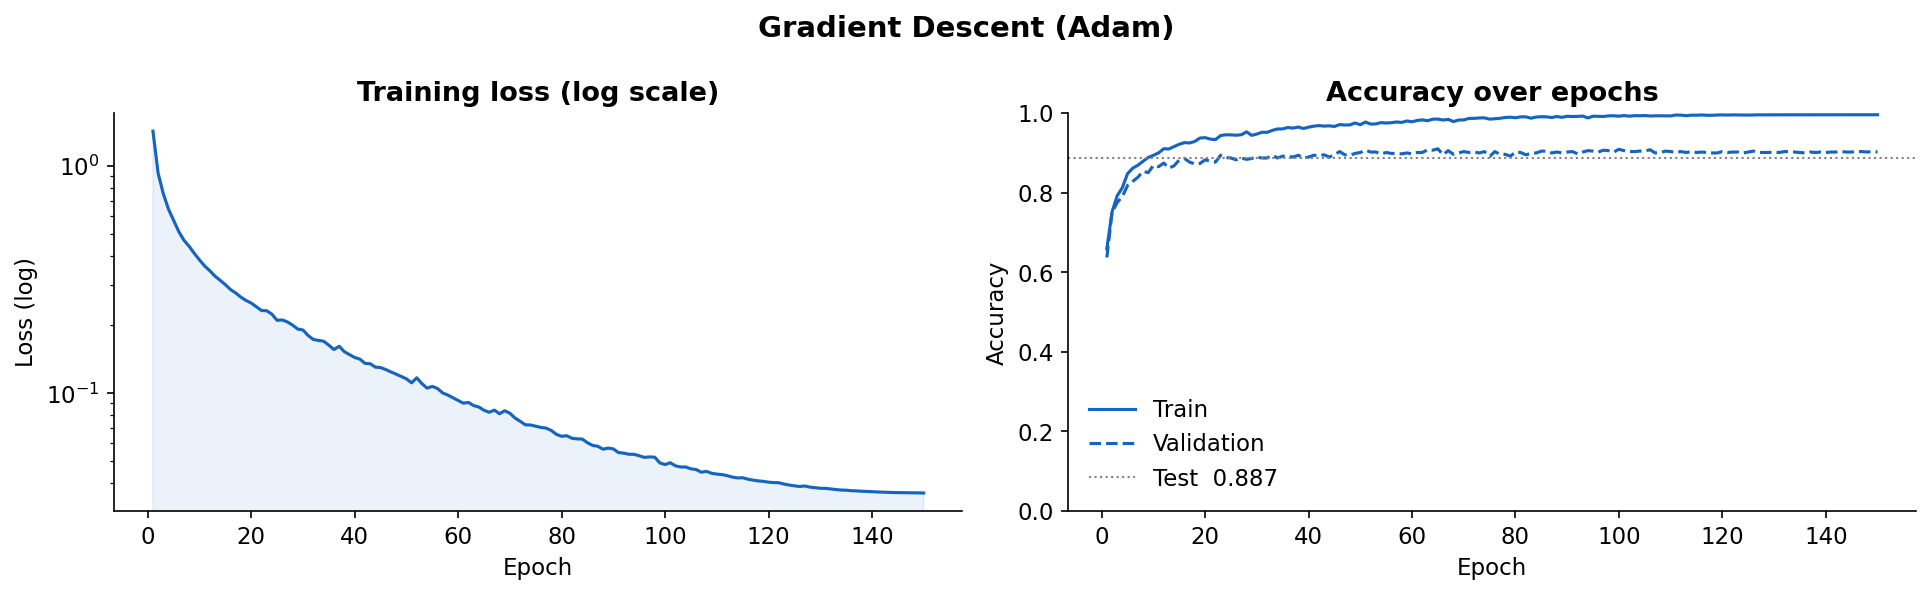
\includegraphics[width=0.85\textwidth]{gd_curves.png}
    \caption{GD training and validation loss/accuracy curves over 150 epochs.}
    \label{fig:gd_curves}
\end{figure}

\subsection{Genetic Algorithm (GA)}

The GA optimises the same 2,710-weight vector without any gradient information. The DEAP library
is used for its clean separation of operator configuration and execution, and safe fitness
invalidation after crossover/mutation.

\paragraph{Encoding.} Each individual is a flat Python list of 2,710 floats, initialised from
$\mathcal{U}(-0.1, 0.1)$ to match PyTorch's default weight scale.

\paragraph{Fitness.} Negative validation accuracy (so DEAP maximises the correct quantity):
$f = -\mathrm{acc}_\mathrm{val}$.

\paragraph{Operators (tuned by Optuna, 20 trials):}
\begin{itemize}
    \item \textbf{Selection:} Tournament selection (size 5).
    \item \textbf{Crossover (BLX-$\alpha$):} $\alpha = 0.5$, applied with probability $p_c = 0.719$.
    \item \textbf{Mutation:} Gaussian perturbation ($\mu=0$, $\sigma=0.05$, per-gene
          prob 0.05), applied with $p_m = 0.045$.
    \item \textbf{Elitism:} Top 1 individual carried forward each generation.
    \item \textbf{Population:} 100 individuals; early stopping with patience 50 generations.
\end{itemize}

To reduce runtime, fitness is evaluated on the 867 validation samples rather than the 6,072
training samples — a $7\times$ speedup per evaluation with negligible effect on selection pressure.

\begin{figure}[H]
    \centering
    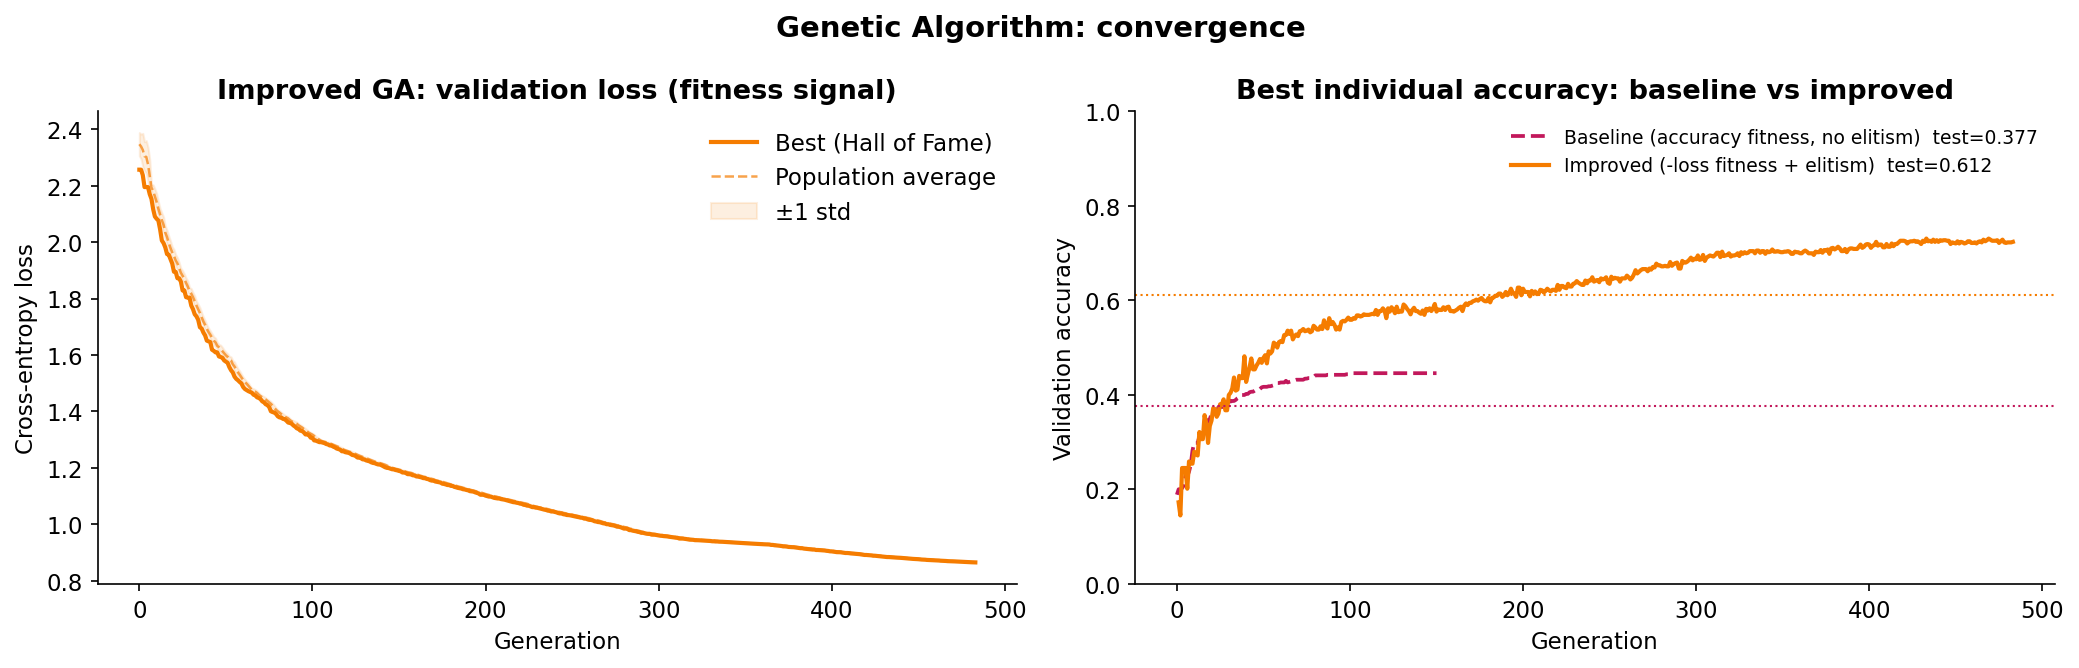
\includegraphics[width=0.85\textwidth]{ga_convergence.png}
    \caption{GA best-fitness progression over generations. The dashed line marks GD's test
    accuracy as a reference ceiling. Early stopping triggered at generation 483.}
    \label{fig:ga_conv}
\end{figure}

% ─────────────────────────────────────────────────────────────────────────────
\section{Hyperparameter Tuning}
% ─────────────────────────────────────────────────────────────────────────────

Optuna with the Tree-structured Parzen Estimator (TPE) is employed for both methods. TPE models
the objective as $p(x \mid y < y^*)$ and $p(x \mid y \geq y^*)$ using kernel density estimates,
then samples from the ratio $\ell(x)/g(x)$ to propose the next trial. \texttt{MedianPruner}
terminates trials whose intermediate validation accuracy falls below the median at each checkpoint,
avoiding wasted computation on clearly unpromising configurations.

\begin{itemize}
    \item \textbf{GD (60 trials):} searches learning rate $[10^{-4}, 10^{-2}]$, weight decay
          $[10^{-6}, 10^{-3}]$, and hidden dimension $\{45, 50, 55, 60, 65\}$.
          Best: $\eta=4.96\!\times\!10^{-3}$, $\lambda=3.29\!\times\!10^{-5}$, $h=60$
          (val acc 91.9\%).
    \item \textbf{GA (20 trials):} searches population size $\{50,75,100,150,200\}$, crossover
          prob $[0.5, 0.9]$, mutation prob $[0.01, 0.2]$, elite count $\{1,2,3,5,8\}$.
          Best: pop=100, $p_c=0.719$, $p_m=0.045$, elite=1.
\end{itemize}

\begin{figure}[H]
    \centering
    \begin{subfigure}[b]{0.48\textwidth}
        \centering
        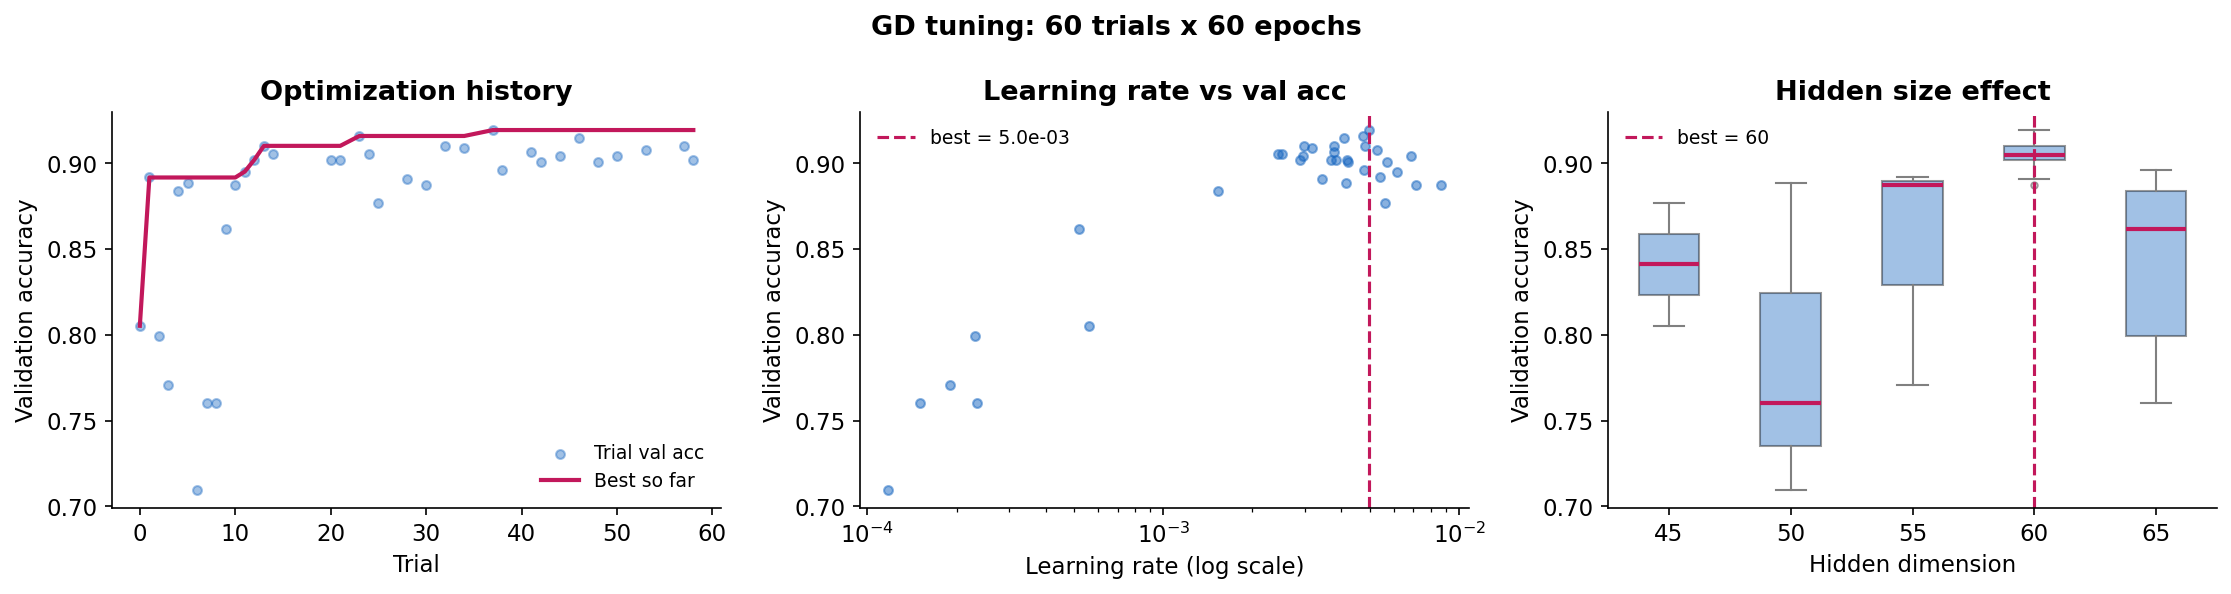
\includegraphics[width=\textwidth]{tuning_gd_optuna.png}
        \caption{GD Optuna optimisation history.}
    \end{subfigure}
    \hfill
    \begin{subfigure}[b]{0.48\textwidth}
        \centering
        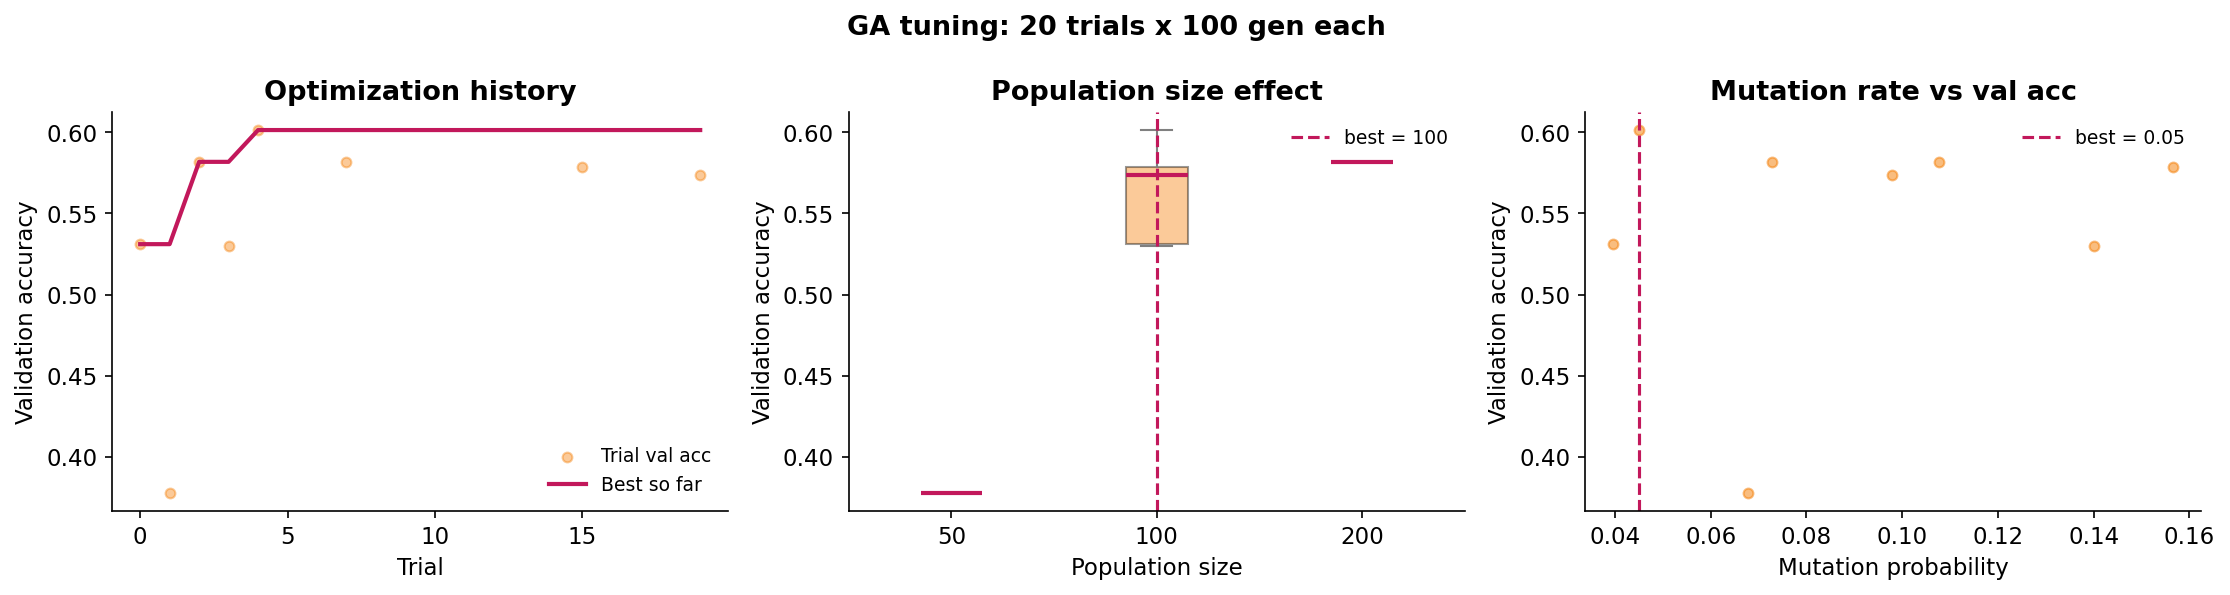
\includegraphics[width=\textwidth]{tuning_ga_optuna.png}
        \caption{GA Optuna optimisation history.}
    \end{subfigure}
    \caption{Hyperparameter tuning results. GD convergence is clear; GA exhibits noisy,
    flat improvement — typical of sparse search in a high-dimensional, non-convex landscape.}
    \label{fig:tuning}
\end{figure}

\begin{figure}[H]
    \centering
    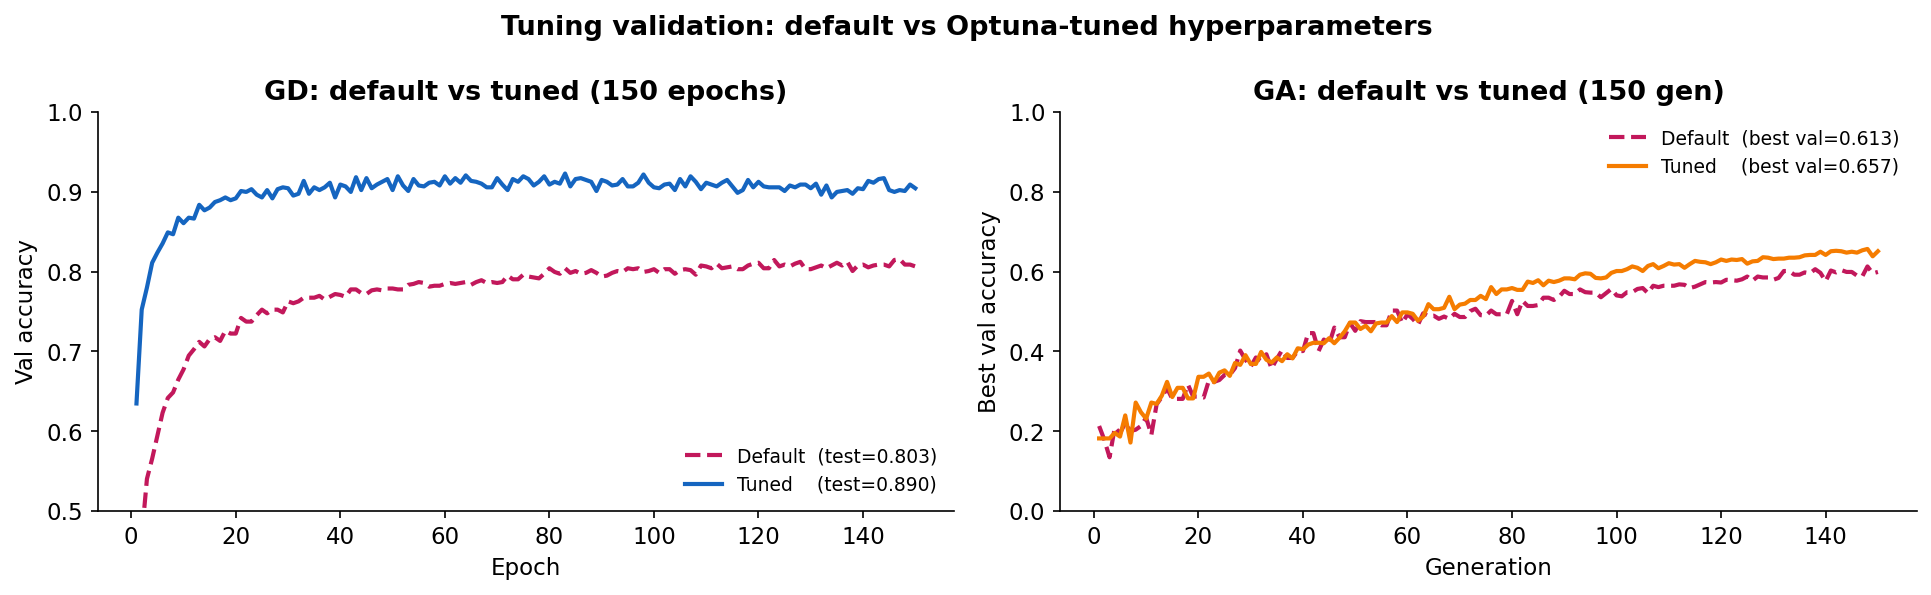
\includegraphics[width=0.75\textwidth]{tuning_validation.png}
    \caption{Default vs tuned validation accuracy. GD improves markedly (default $h=20$,
    $\eta=10^{-3}$ baseline $\approx$81\% $\to$ tuned 91.9\%). GA shows modest gains.}
    \label{fig:tuning_val}
\end{figure}

% ─────────────────────────────────────────────────────────────────────────────
\section{Evaluation and Comparison}
% ─────────────────────────────────────────────────────────────────────────────

Both tuned models are evaluated on the held-out test set (1,734 samples). Results are summarised
in Table~\ref{tab:results}.

\begin{table}[H]
    \centering
    \caption{Test-set performance comparison.}
    \label{tab:results}
    \begin{tabular}{lcccc}
        \toprule
        Method & Test Acc & Macro F1 & Time (s) & Epochs/Gen \\
        \midrule
        GD (Adam, tuned) & 88.7\% & 0.887 & $\approx$52 & 150 epochs \\
        GA (DEAP, tuned) & 61.2\% & 0.614 & $\approx$155 & 483 gen \\
        GA (default, untuned) & 37.7\% & --- & --- & 150 gen \\
        \bottomrule
    \end{tabular}
\end{table}

\begin{figure}[H]
    \centering
    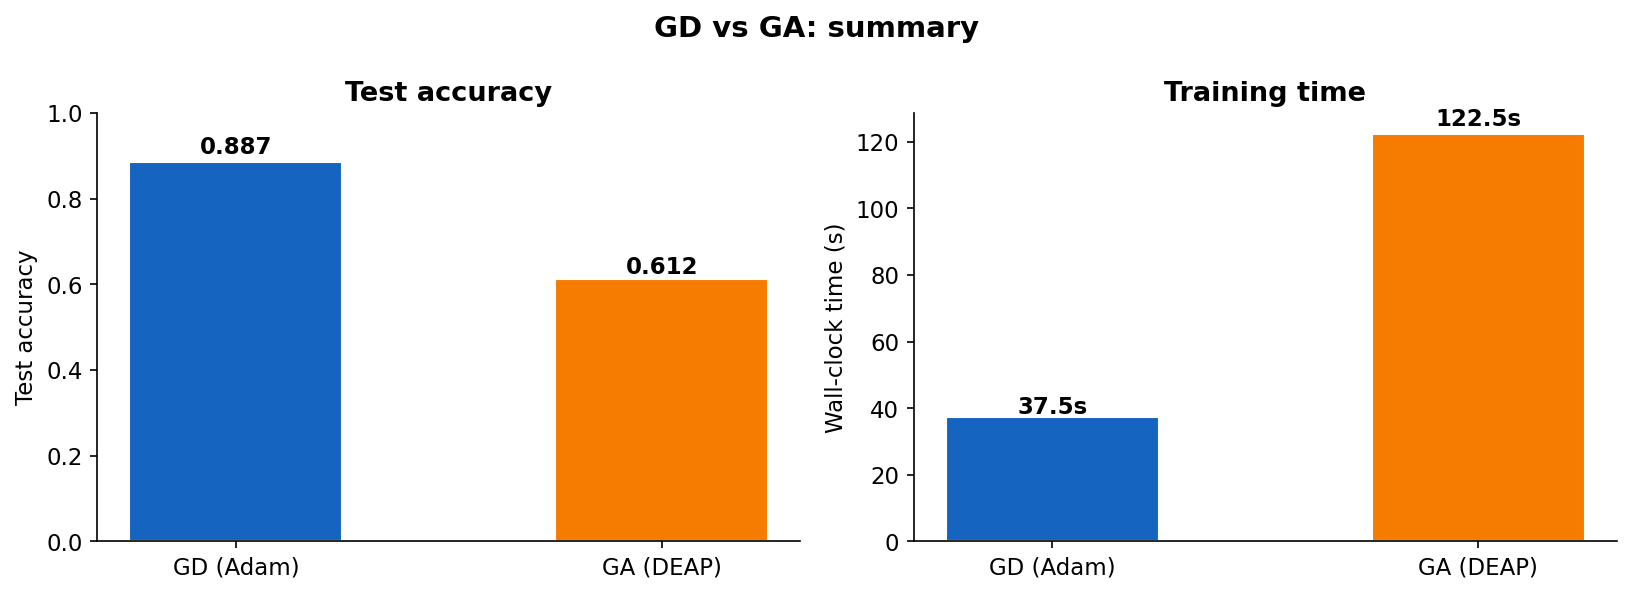
\includegraphics[width=0.85\textwidth]{comparison_summary.png}
    \caption{Summary comparison of accuracy and training time.}
    \label{fig:summary}
\end{figure}

\begin{figure}[H]
    \centering
    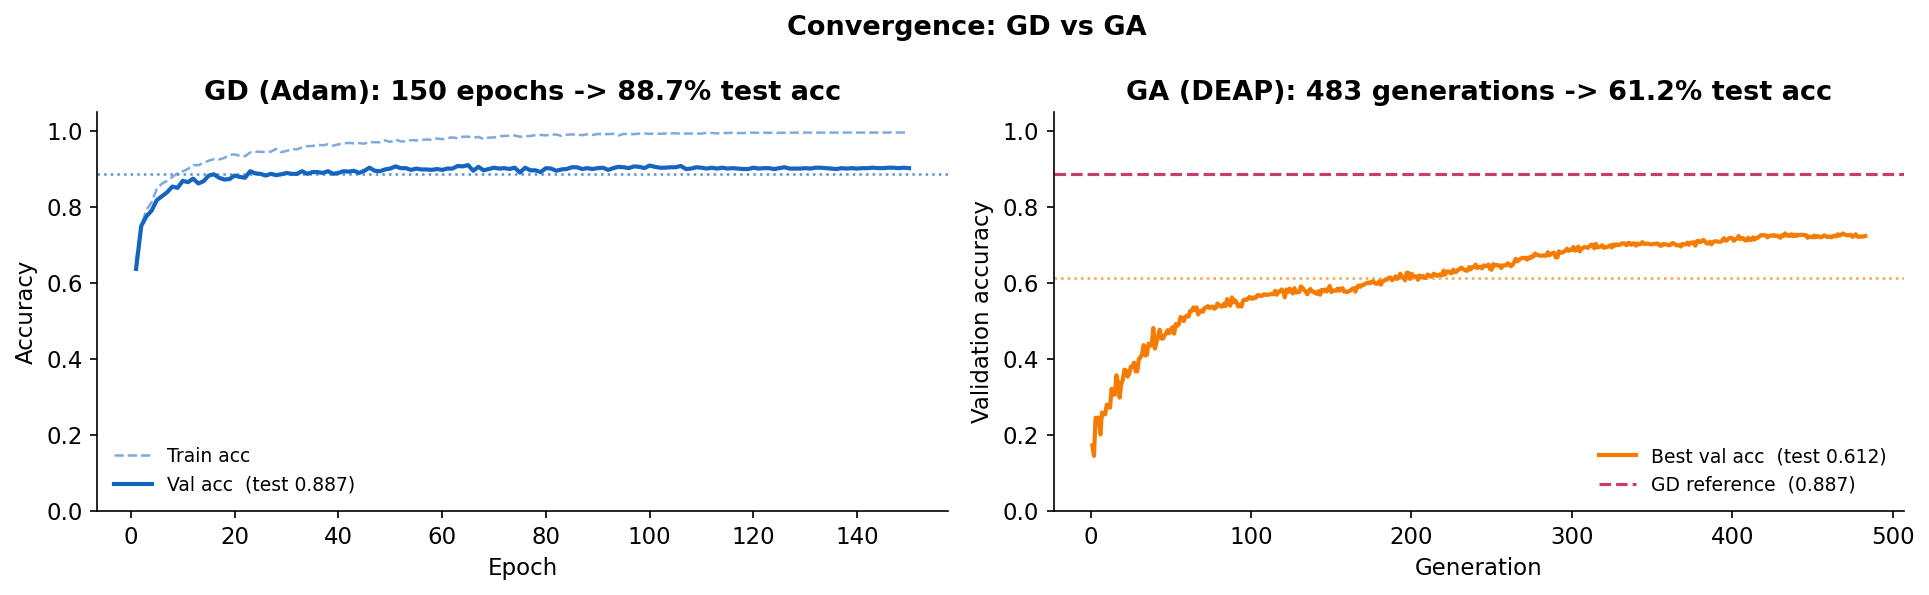
\includegraphics[width=\textwidth]{comparison_convergence.png}
    \caption{Convergence plots. Left panel: GD loss and accuracy over 150 epochs.
    Right panel: GA best fitness over generations (pink dashed = GD test accuracy reference).
    Independent x-axes preserve the natural scale of each method.}
    \label{fig:convergence}
\end{figure}

\begin{figure}[H]
    \centering
    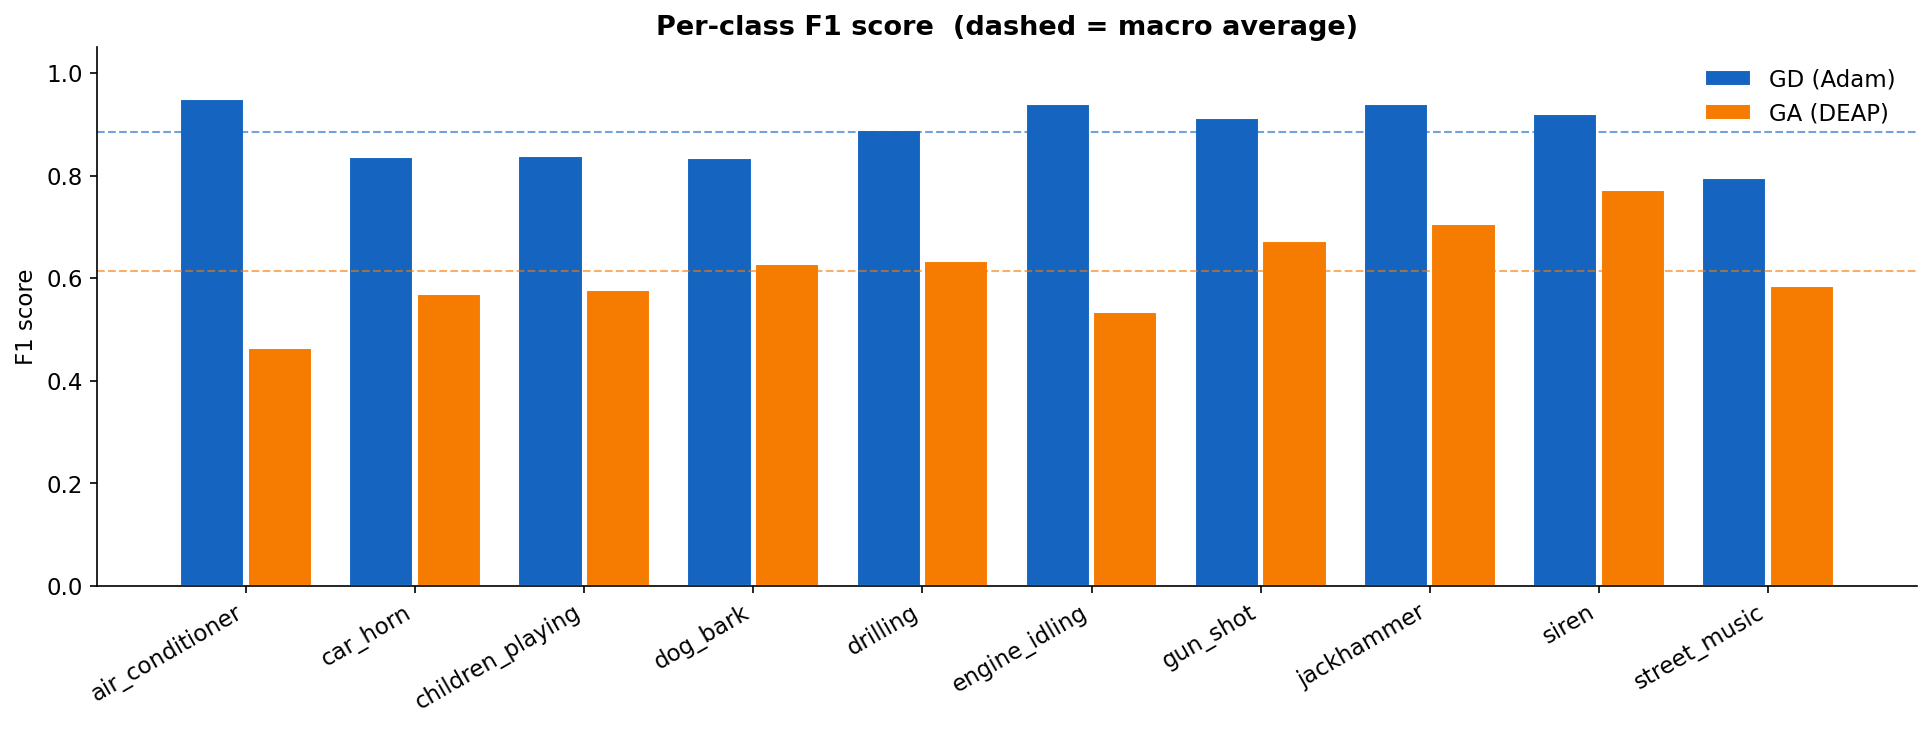
\includegraphics[width=0.85\textwidth]{comparison_f1.png}
    \caption{Per-class F1 scores. GD achieves consistently high F1 across all 10 classes.
    GA shows class-specific variation reflecting the noisier fitness landscape.}
    \label{fig:f1}
\end{figure}

\begin{figure}[H]
    \centering
    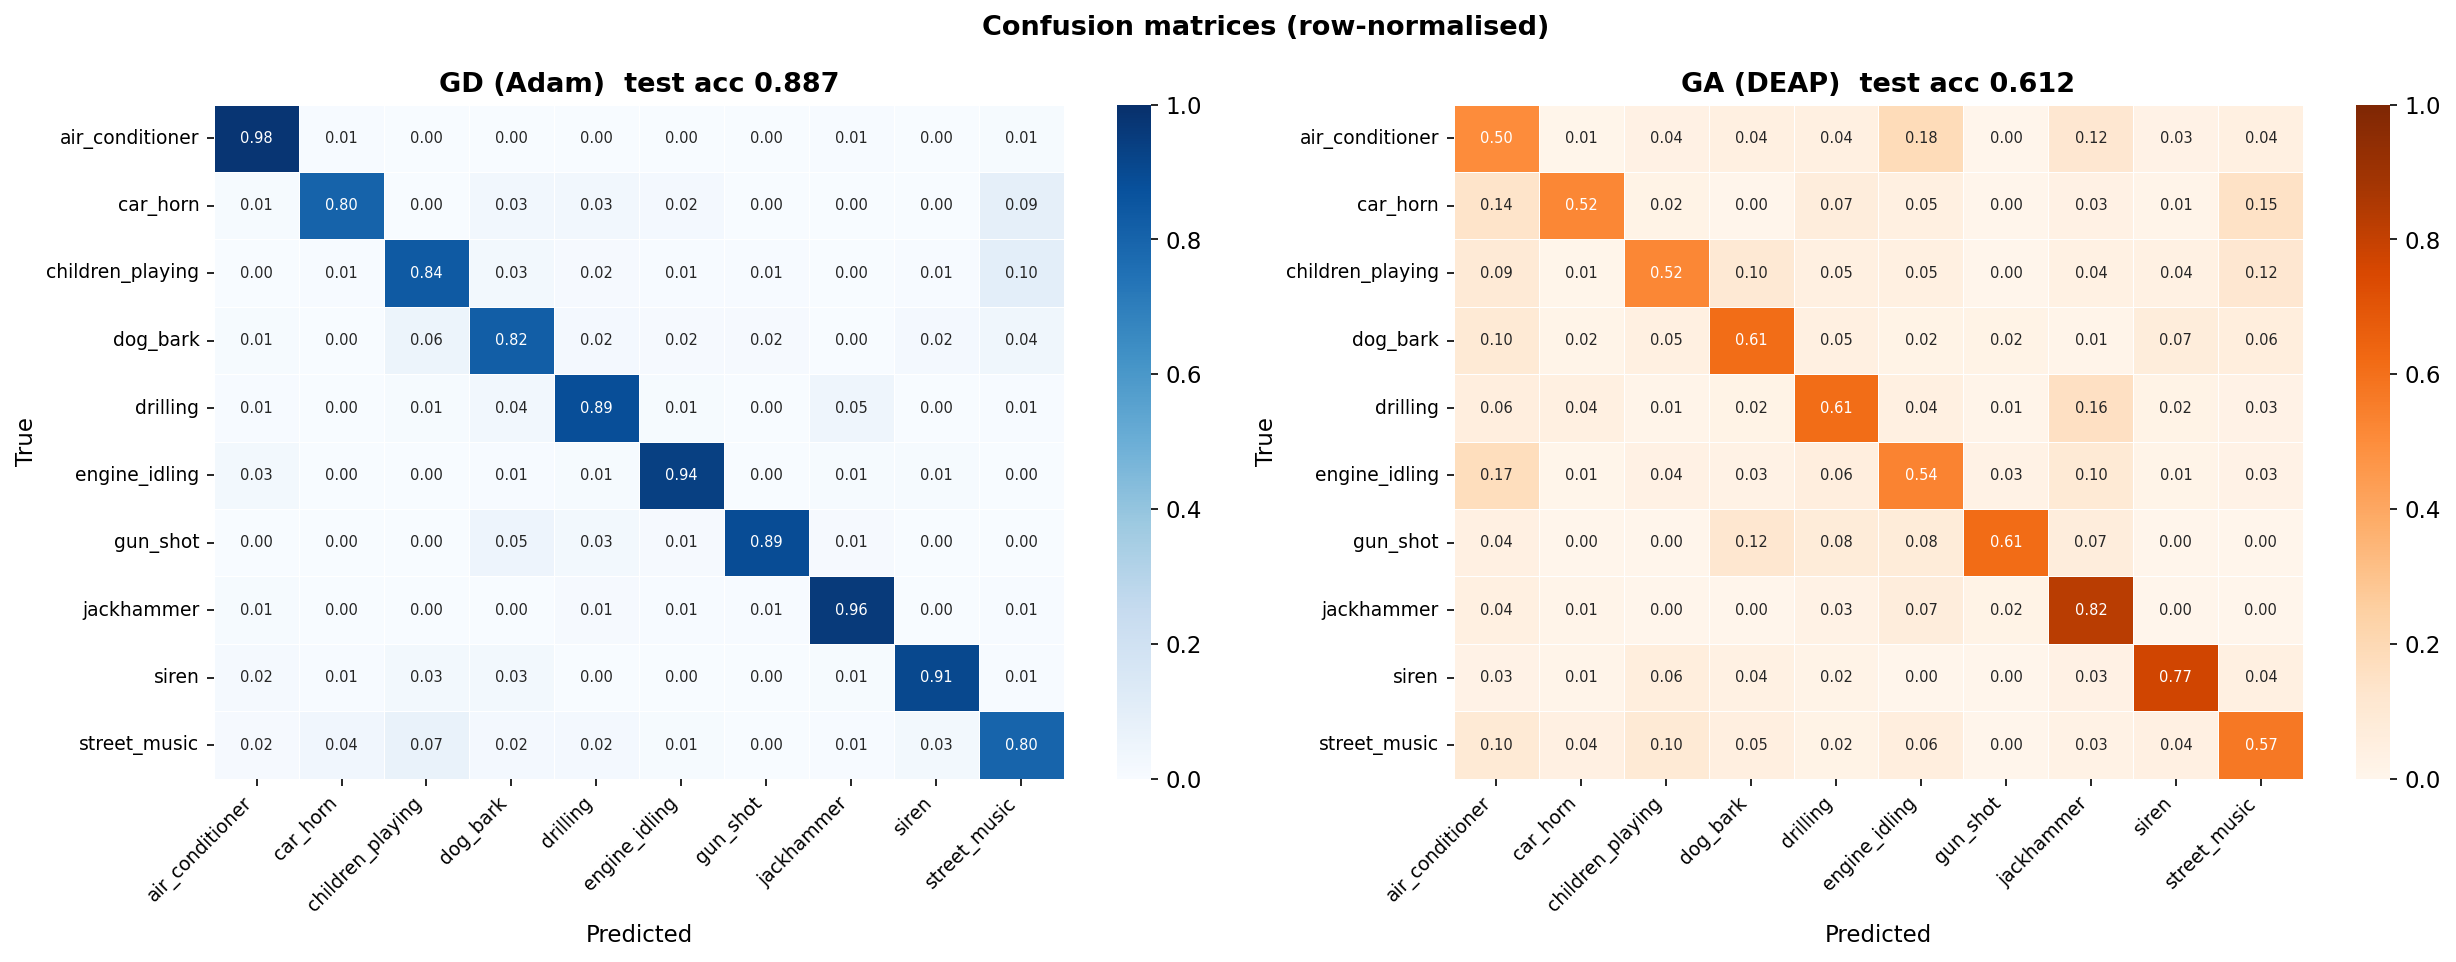
\includegraphics[width=\textwidth]{comparison_confusion.png}
    \caption{Normalised confusion matrices. GD (left) shows mostly diagonal predictions.
    GA (right) exhibits more off-diagonal confusion, particularly for acoustically similar
    classes.}
    \label{fig:confusion}
\end{figure}

% ─────────────────────────────────────────────────────────────────────────────
\section{Conclusion}
% ─────────────────────────────────────────────────────────────────────────────

GD with Adam is significantly more effective for training this MLP: 88.7\% test accuracy vs.\
61.2\% for the GA, achieved in one-third the wall-clock time (52s vs.\ 155s). The key structural
advantage of GD is that backpropagation computes the gradient for all 2,710 weights in a single
forward-backward pass. The GA must evaluate the entire population ($\sim$100 individuals) to
produce a single generation's update — with no guarantee of monotone improvement.

The GA's competitive strength lies in being gradient-free: it can in principle optimise any
non-differentiable objective over any search space. However, for a smooth, differentiable MLP
loss with 2,710 continuous parameters, the GA's population-based exploration is simply
outmatched by gradient information.

The tuning results reinforce this: GD improved from $\approx$81\% to 88.7\% on test
(+11 pp) with 60 Optuna trials, while the GA's improvement was marginal and noisy across 20
trials, reflecting a flat, stochastic fitness landscape where small configuration changes have
unpredictable effects.

\end{document}
